% ── Anexo A: Código fuente y datos ───────────────────────────────────────────
\chapter{Código fuente y datos analizados}
\label{anexo:codigo}

El código fuente completo desarrollado durante este trabajo se encuentra disponible en el siguiente repositorio de GitHub:

\begin{center}
\url{https://github.com/jmmachadol/tfm_FP-A}
\end{center}

\section*{Estructura del repositorio}

\begin{itemize}
  \item \texttt{src/} — módulos Python del \textit{pipeline}:
    \begin{itemize}
      \item \texttt{config.py} — parámetros del experimento, semillas y rutas relativas.
      \item \texttt{utils.py} — fijación de semillas globales y sistema de \textit{logging}.
      \item \texttt{data\_loader.py} — descarga con caché del M4 Financial Monthly.
      \item \texttt{preprocessor.py} — filtrado, submuestra estratificada, escalado.
      \item \texttt{backtesting.py} — motor walk-forward y verificador de leakage.
      \item \texttt{evaluation.py} — las seis métricas de evaluación validadas con tests.
      \item \texttt{visualization.py} — generación de las cinco figuras del experimento.
      \item \texttt{models/} — una implementación por familia de modelos (\texttt{base.py}, \texttt{baseline.py}, \texttt{statistical.py}, \texttt{ml.py}).
    \end{itemize}
  \item \texttt{notebooks/main.ipynb} — cuaderno orquestador; importa los módulos anteriores sin contener lógica de negocio \textit{inline}.
  \item \texttt{run\_experiment.py} — script autónomo equivalente al cuaderno, con argumentos configurables (\texttt{--n-series}, \texttt{--max-folds}).
  \item \texttt{tests/} — pruebas automatizadas: \texttt{test\_evaluation.py} (14 pruebas, métricas validadas contra cálculo manual) y \texttt{test\_backtesting.py} (6 pruebas, incluye detección de leakage inyectado).
  \item \texttt{results/} — tablas de resultados en CSV y figuras en PNG generadas por el experimento.
  \item \texttt{requirements.txt} — dependencias exactas del entorno de ejecución.
  \item \texttt{data/raw/} — los datos del M4 se descargan automáticamente al primer uso del módulo \texttt{data\_loader.py} desde el repositorio oficial de la competición M4.
\end{itemize}

\section*{Diagrama de arquitectura del \textit{pipeline}}

La Figura~\ref{fig:diagrama_pipeline} presenta la arquitectura modular del \textit{pipeline} desarrollado, mostrando el flujo de datos desde la carga del dataset hasta la generación de los resultados comparativos.

\begin{figure}[H]
\caption{\textbf{Figura A.1.} \textit{Diagrama de flujo del pipeline de pronóstico para FP\&A. Se distinguen cuatro bloques funcionales: adquisición y preprocesamiento de datos, generación del protocolo walk-forward, ajuste e inferencia de los siete modelos, y evaluación con las seis métricas. El cuaderno orquestador coordina la ejecución integrada de todos los módulos.}}
\label{fig:diagrama_pipeline}
\vspace{4pt}
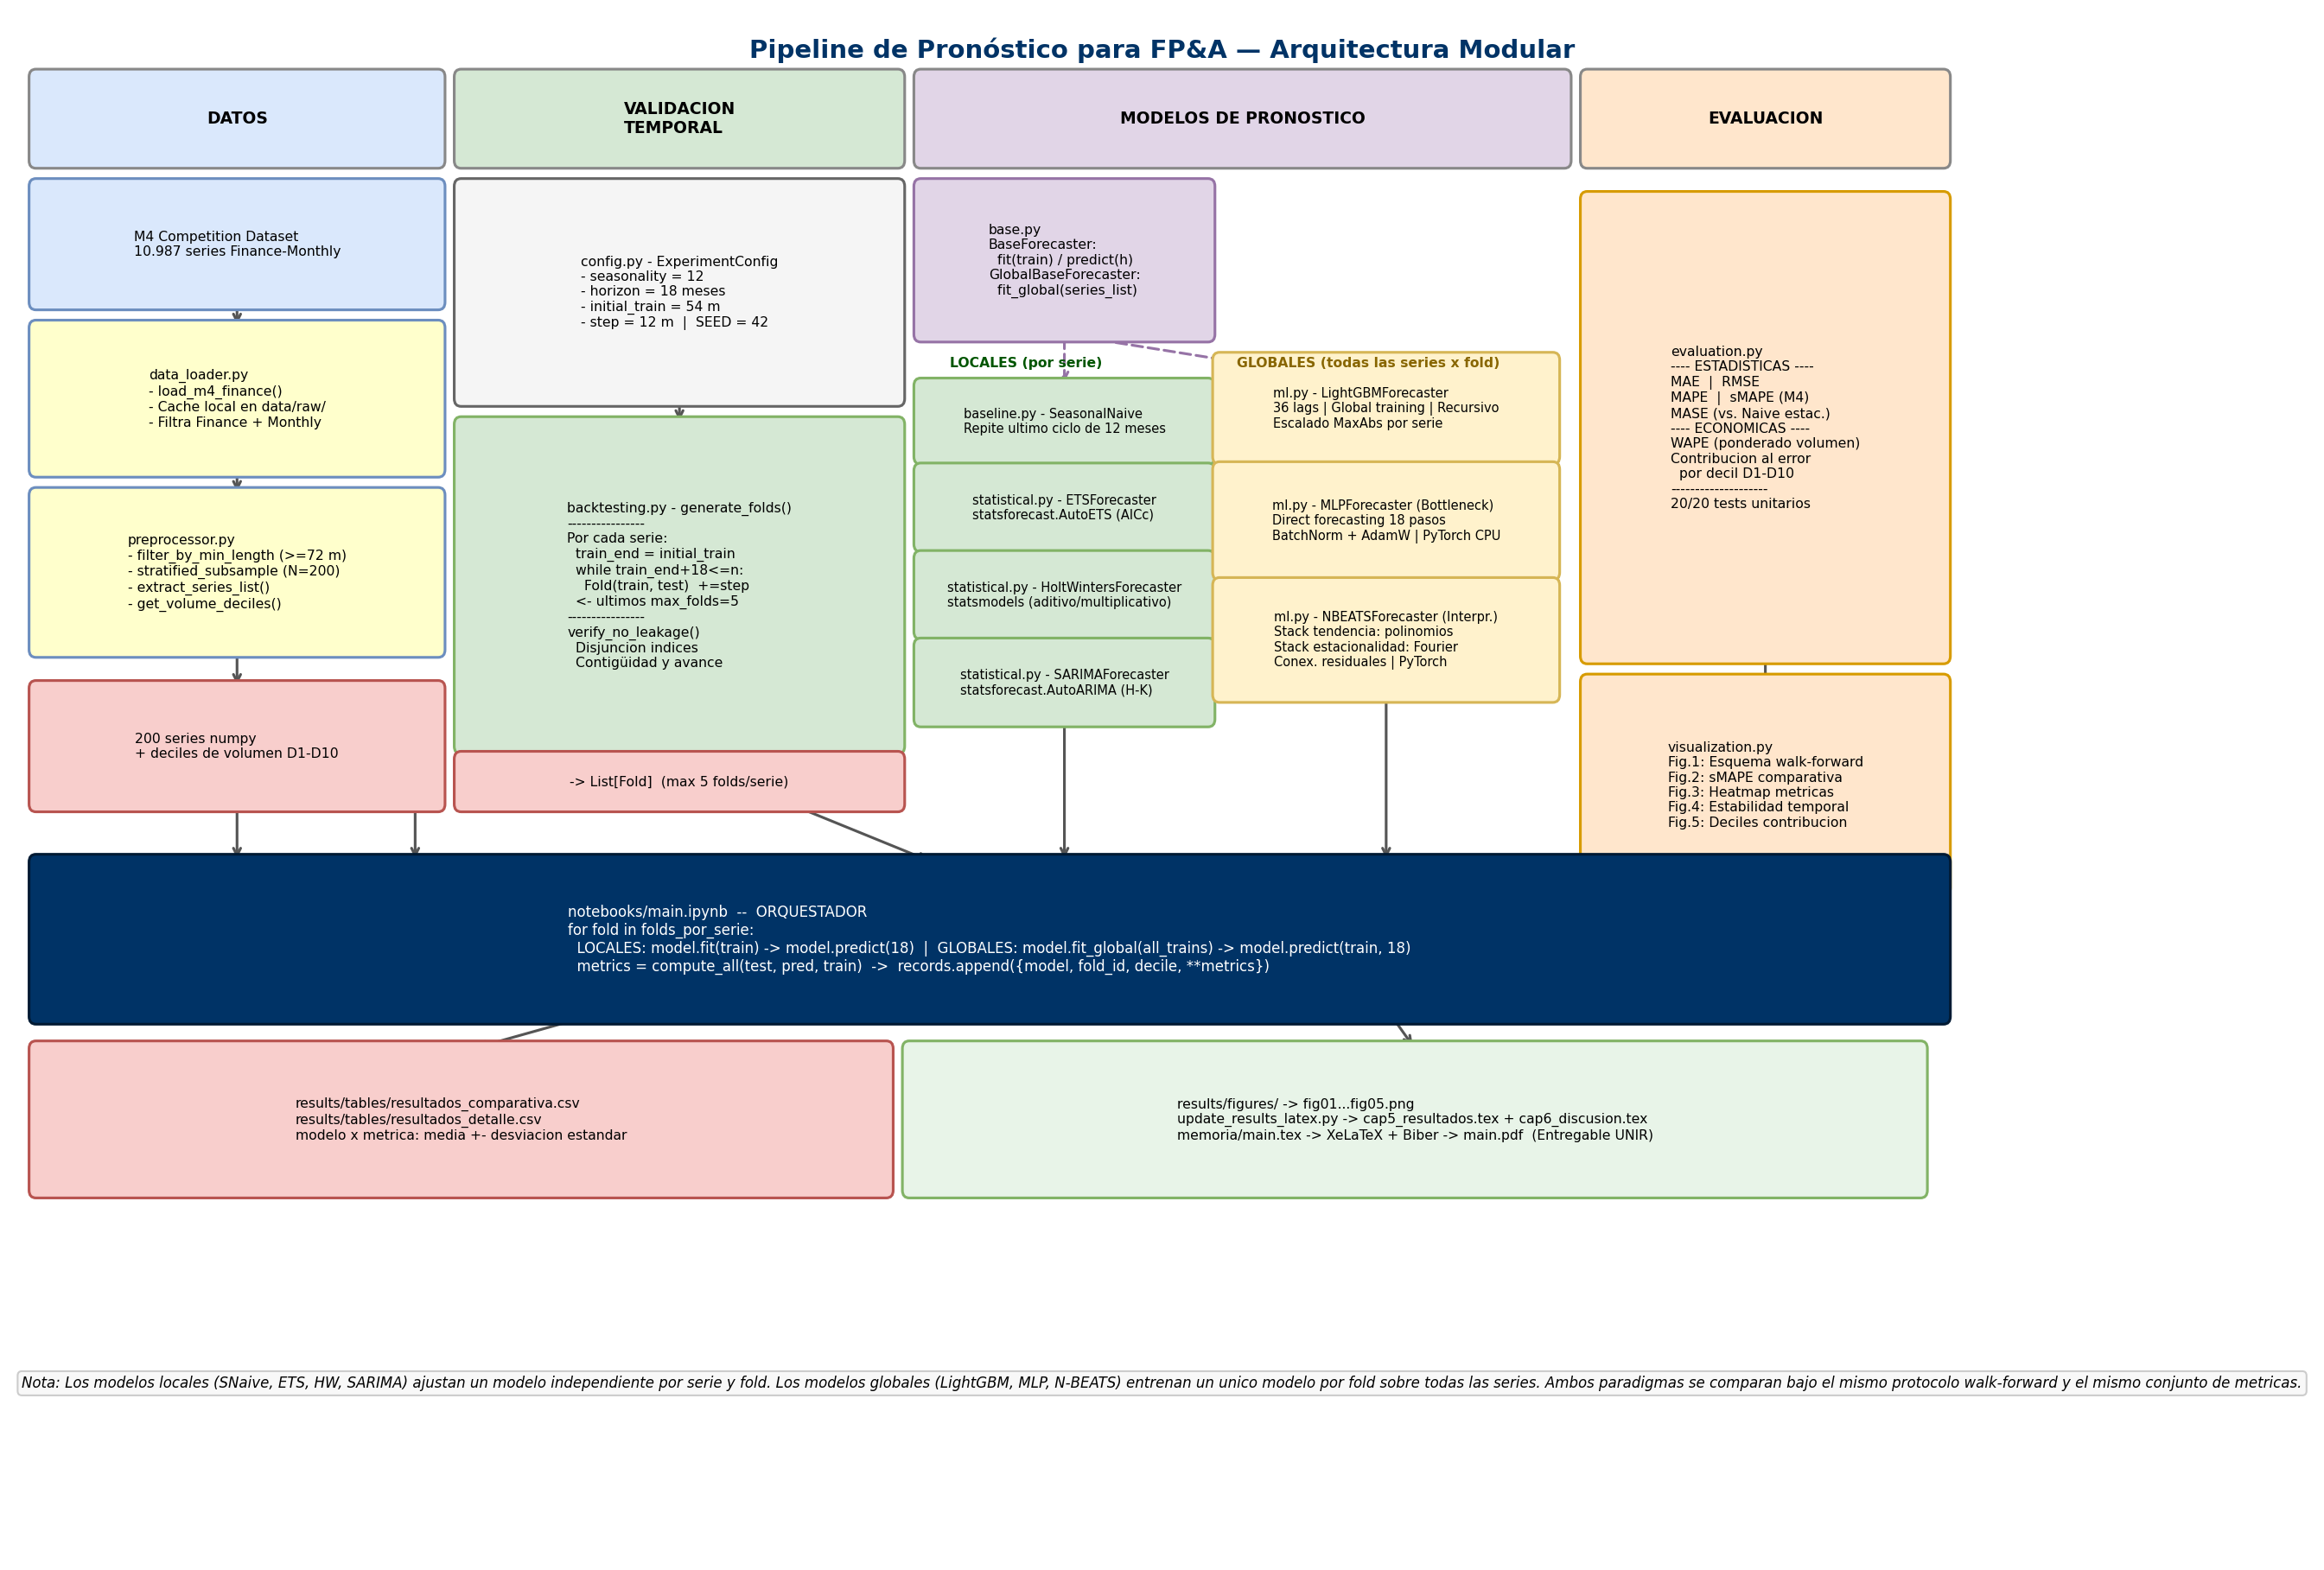
\includegraphics[width=\textwidth]{figuras/diagrama_pipeline.png}
\vspace{4pt}

\small\textit{Fuente: elaboración propia.}
\end{figure}

Los autores son los únicos propietarios del repositorio y únicos responsables del código fuente. Los datos utilizados son de acceso público (M4 Competition Dataset) y están disponibles en el repositorio oficial de la competición M4 (\url{https://github.com/Mcompetitions/M4-methods}).

\textbf{Nota de confidencialidad:} este TFE no está asociado a datos internos de ninguna organización. Los datos utilizados son exclusivamente los del conjunto M4, de acceso público.

\section*{Reproducibilidad}

Para reproducir el experimento completo:

\begin{enumerate}
  \item Instalar las dependencias: \texttt{pip install -r requirements.txt}
  \item Ejecutar: \texttt{python run\_experiment.py --n-series 200 --max-folds 5}
  \item Actualizar la memoria con los resultados: \texttt{python update\_results\_latex.py}
  \item Compilar el documento: \texttt{cd memoria \&\& latexmk -xelatex main.tex}
\end{enumerate}

El módulo \texttt{src/utils.py} fija las semillas de NumPy, PyTorch y el módulo \texttt{random} de la biblioteca estándar antes de cualquier operación aleatoria, garantizando resultados idénticos entre ejecuciones.
